\documentclass{article}

\usepackage[utf8]{inputenc}
\usepackage{graphicx}		% Graphics.
\usepackage{color}
\usepackage[english]{babel}
\usepackage{float}
\usepackage{subcaption}
\usepackage{xfrac}
\usepackage{matlab-prettifier}
\usepackage{amsmath}    
\usepackage{amssymb}
\usepackage{siunitx}
\usepackage{pdfpages}
\usepackage{hyperref}
\usepackage{longtable}
\usepackage{multicol}
\usepackage{enumitem}

% Create a separate table for the appendix.
\usepackage[toc,page]{appendix}

% Table of Content has fast links to sections.
\usepackage{hyperref}

% Remove dots in table of contents.
\usepackage[titles]{tocloft}
\renewcommand{\cftdot}{}

% Page style.
\usepackage[top=2cm, bottom=2cm, left = 2cm, right = 2cm]{geometry}
\setlength{\parindent}{0pt}	% Disable indents.

\begin{document}
	
	%----------------------------------------------------------------------------------------
	%	Title page.
	%----------------------------------------------------------------------------------------
	\begin{titlepage}
		\center
		\newcommand{\HRule}{\rule{\linewidth}{0.5mm}}
			\textsc{\Huge Battle of the Neighbourhoods}\\[1.5cm]
			\textsc{\LARGE Applied Data Capstone - Coursera}\\[0.3cm]
			\textsc{\large Diego Talavera}\\[0.5cm]
		\vspace{3cm}
		\textsc{\LARGE Github link to Jupyter Notebook:\\ \url{https://github.com/dtalavera8/Coursera_Capstone/blob/master/BattleOfTheNeighborhoods.ipynb}}
			\vfill\vfill\vfill % Position the date 3/4 down the remaining page.
			
			{\large\today} % Date, change the \today to a set date if you want to be precise.
	\end{titlepage}
	
	
	%----------------------------------------------------------------------------------------
	%	TABLE OF CONTENT.
	%----------------------------------------------------------------------------------------
	\newpage				% Start at new page.
	\pagenumbering{arabic}	% Page numbering reset & style.
	\renewcommand{\contentsname}{Table of Contents}
	\tableofcontents		% Add table of content.
	
	%----------------------------------------------------------------------------------------
	% 	INTRODUCTION
	%----------------------------------------------------------------------------------------
	
	\newpage
	\section{Introduction}
	\textbf{NOTE: Unfortunately, folium maps are not displayed through the github website, so they can be seen in this report, although, not interactively.}
	\subsection{Problem Description}
		Imagine that you need to buy a set of items, some of which has to be bought in a few different stores. You want to find a place around your city that has all of these stores you need within a certain short distance from each other. And if there are multiple options, how can you choose which place to select to visit the stores?
	
	\subsection{Description and use of data}
		In this section, the data will be described, as well as some assumptions needed to simplify the analysis. The methods to be used are also presented here. 
		
		\subsubsection{Data descriprion}
		\begin{itemize}
			\item \textbf{Location:} The city selected will be Stockholm, Sweden with the starting point in the city center.
			\item \textbf{Items to buy:} An arbitrary list of items to be bought was created along with the corresponding store category
			\item \textbf{Available Venues:} Information regarding the available stores was obtained through the Foursquare API. The data includes venue category, name, rating, location, and unique ID.				
		\end{itemize}
		\subsubsection{Data usage, assumptions and observations}
			In order to make the data analysis less complicated, some assumptions and considerations are made after a brief look at the data.:
			\begin{itemize}
				\item The starting point of the experiment was at the coordinates provided by geopy for "Stockholm, Sweden"
				\item The distance taken into account was the straight-line distance, so no streets or highways were considered.
				\item Similarly, no traffic data was taken into account			
			\end{itemize} 	
		\newpage
		\subsubsection{Methods - Oveerview}
			First, the required venue categories were obtained from the Foursquare API in order to see all the available venues around our starting point. Once the venues are obtained, a first dataframe with the information was created and then venues were plotted using the folium library in order to see the distribution. 
			
			Afterwards, a couple of machine learning algorithms were used in order to obtain the clusters with the desired characteristics. 
			
			And finally, a simple weighted score was proposed to choose the best cluster to visit
			
\section{Methodology}

	\subsection{Obtaining the data}
		The venue data was obtained through the Foursquare API. Initially, the categories of the stores were used using a search call, but it was discovered that the search call tries to match either fully or partially to venue names, without taking into account the categories.
		Therefore, the venue category IDs were obtained through a different call through the API and then used to retrieve all the venues that the API can provide of each category.
		
		With this information, a dataframe was constructed with the information that was deemed necessary: Venue Name, ID, latitude and longitude and category. These venues were then plotted with Folium in order to visualize all the available locations. In this first visualization, a color was chosen for each venue category to make the understanding of the distribution, easier. 
		\begin{figure}[H]
			\centering
			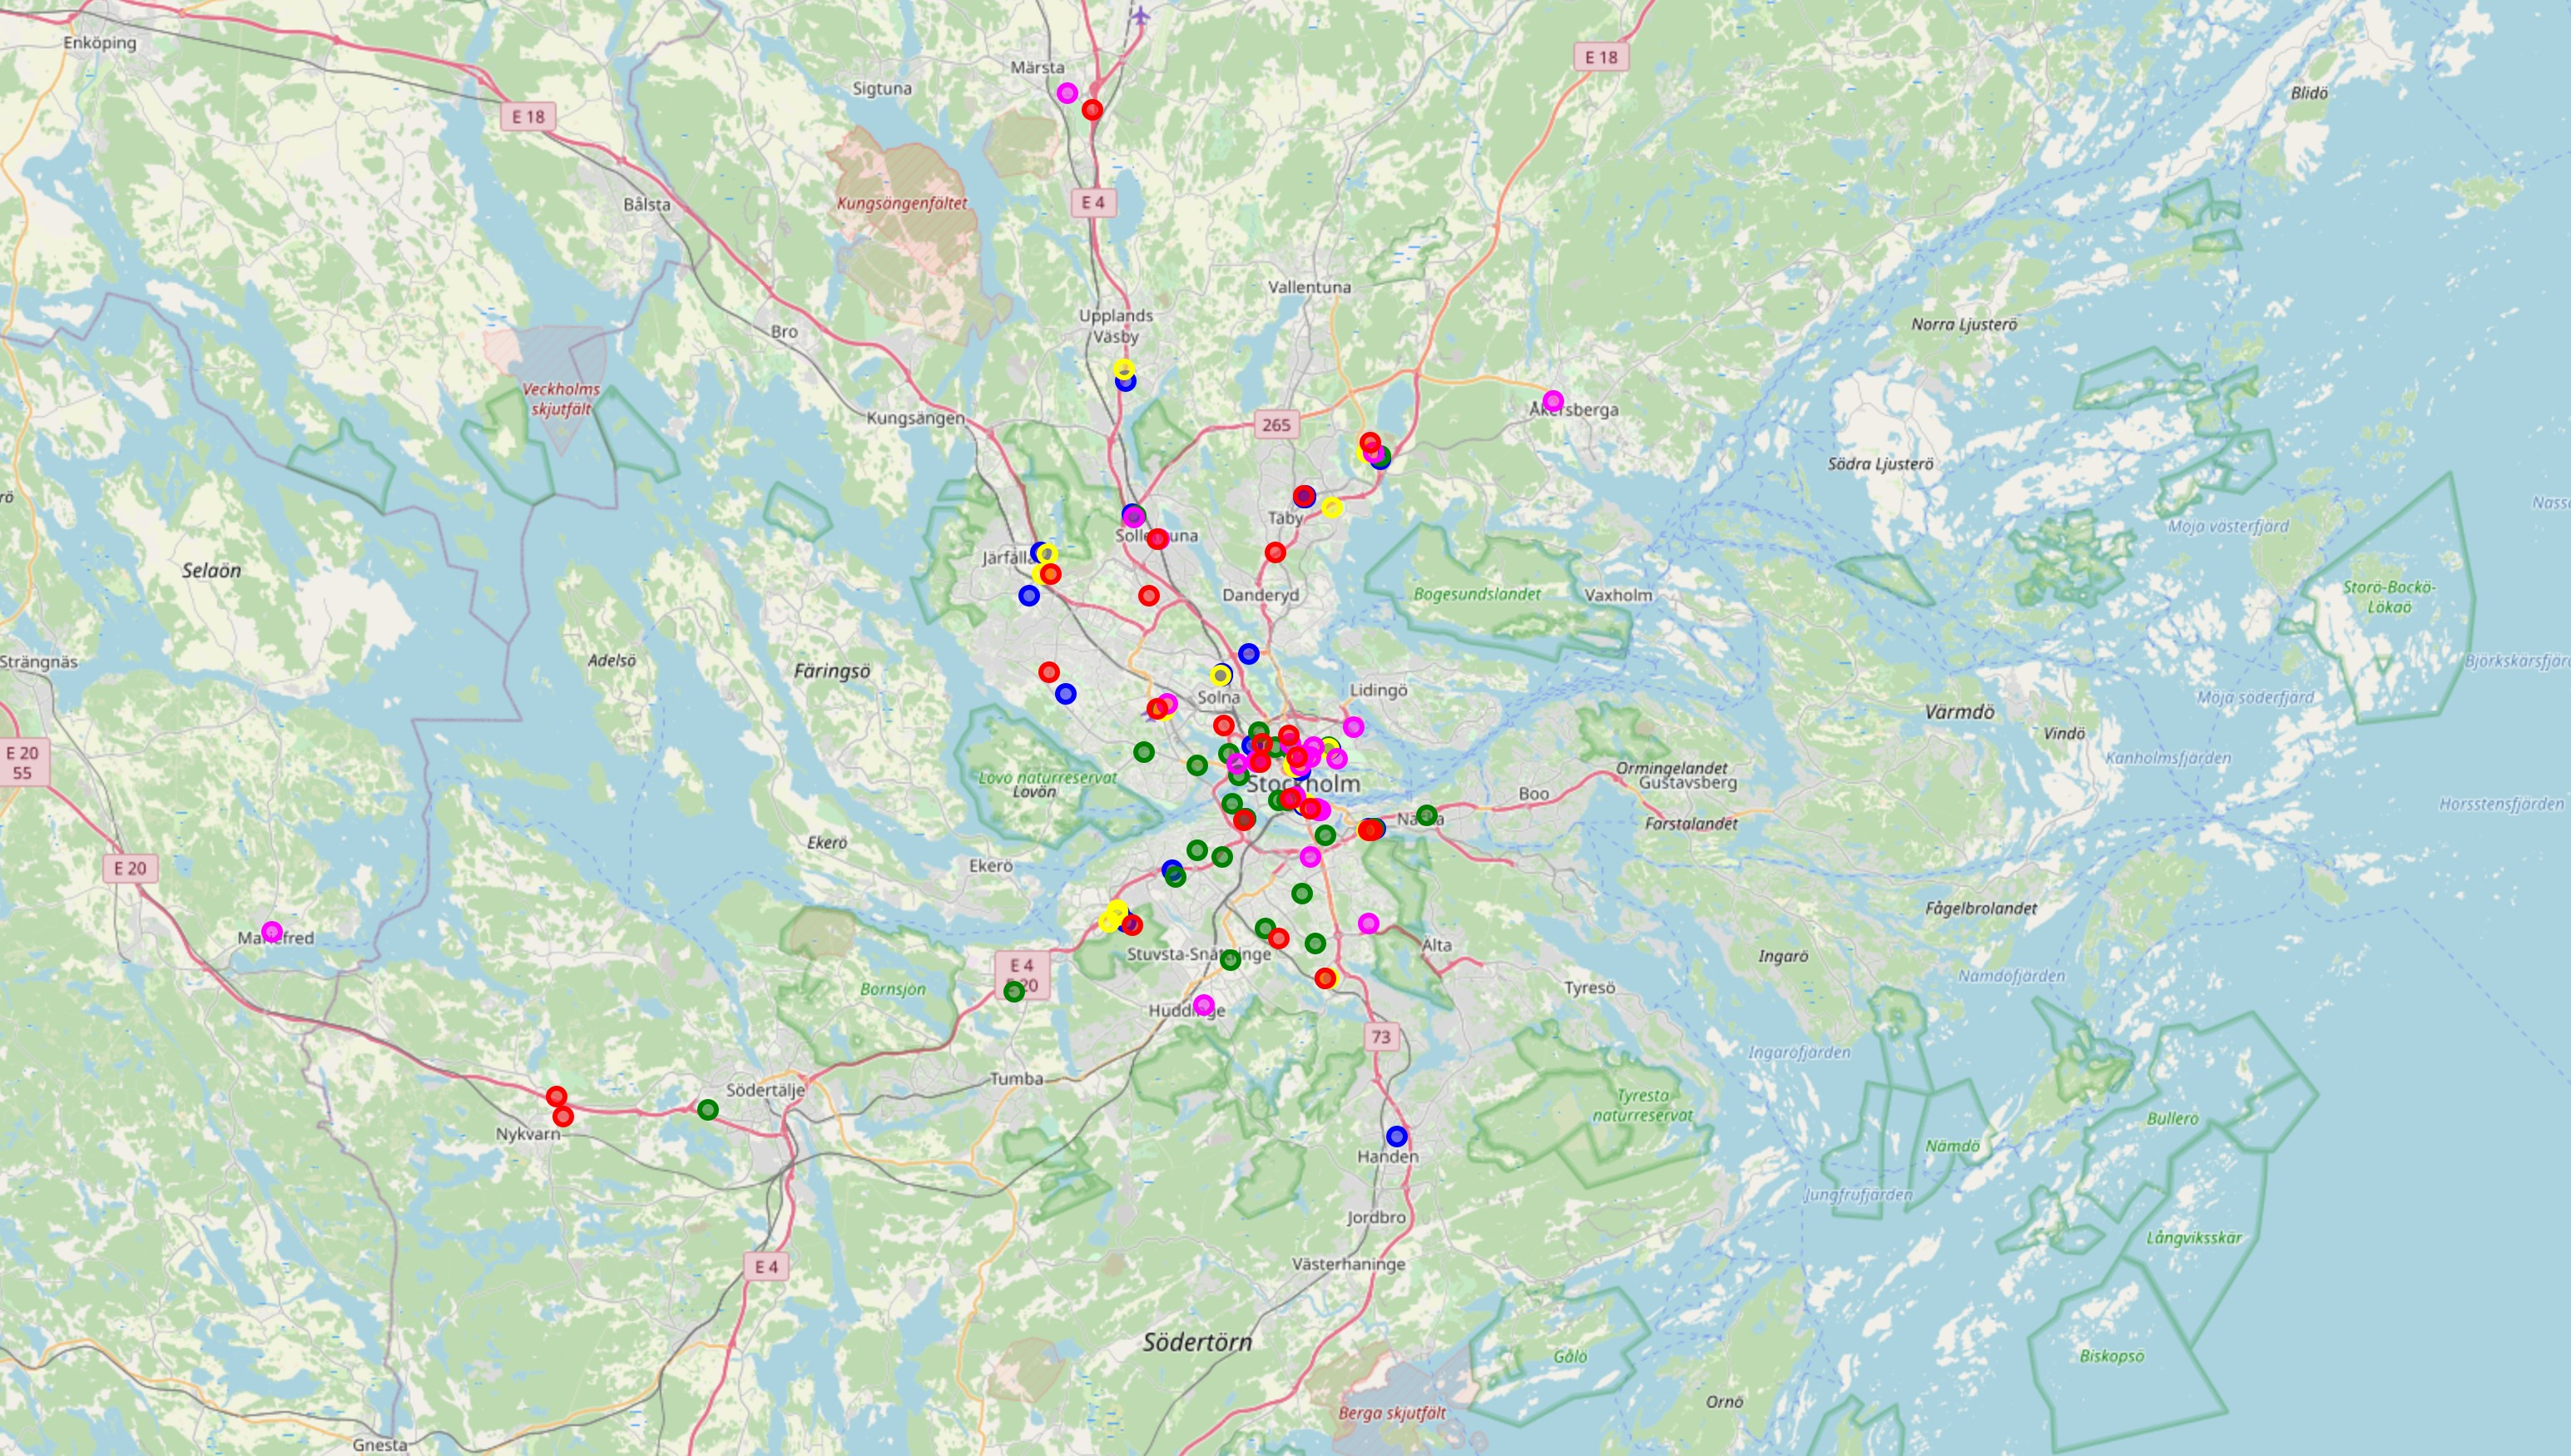
\includegraphics[width=\textwidth]{img/map1.jpg}
			\caption{All the venues obtained from the Foursquare API}
			\label{fig::map1}
		\end{figure}
	\subsection{Exploratory Data Analysis}
	
		A very simple preliminary data analysis was performed at this point. The distance to the start point of the map was calculated for each venue. Then, it was found from the map above (\ref{fig::map1}) that some venues farther away from the start are very scattered, therefore wont be able to form a cluster relevant to us. After a few tries, it was determined that venues with a distance to the start larger than \SI{16.5}{\kilo \meter} were going to be dropped. 
		
	\subsection{Machine learning algorithms}
		At this point, the first machine learning algorithm was chosen and applied. Since we are dealing with a clustering problem. Unsupervised learning was selected, and as a first step, \textbf{K-Means} from the scikit learn was applied to the data. This allowed to very quickly form a few clusters "around" our starting point, effectively creating some zones based on distance from the starting point. The clusters created at this point are as follows:
		\begin{figure}[H]
			\centering
			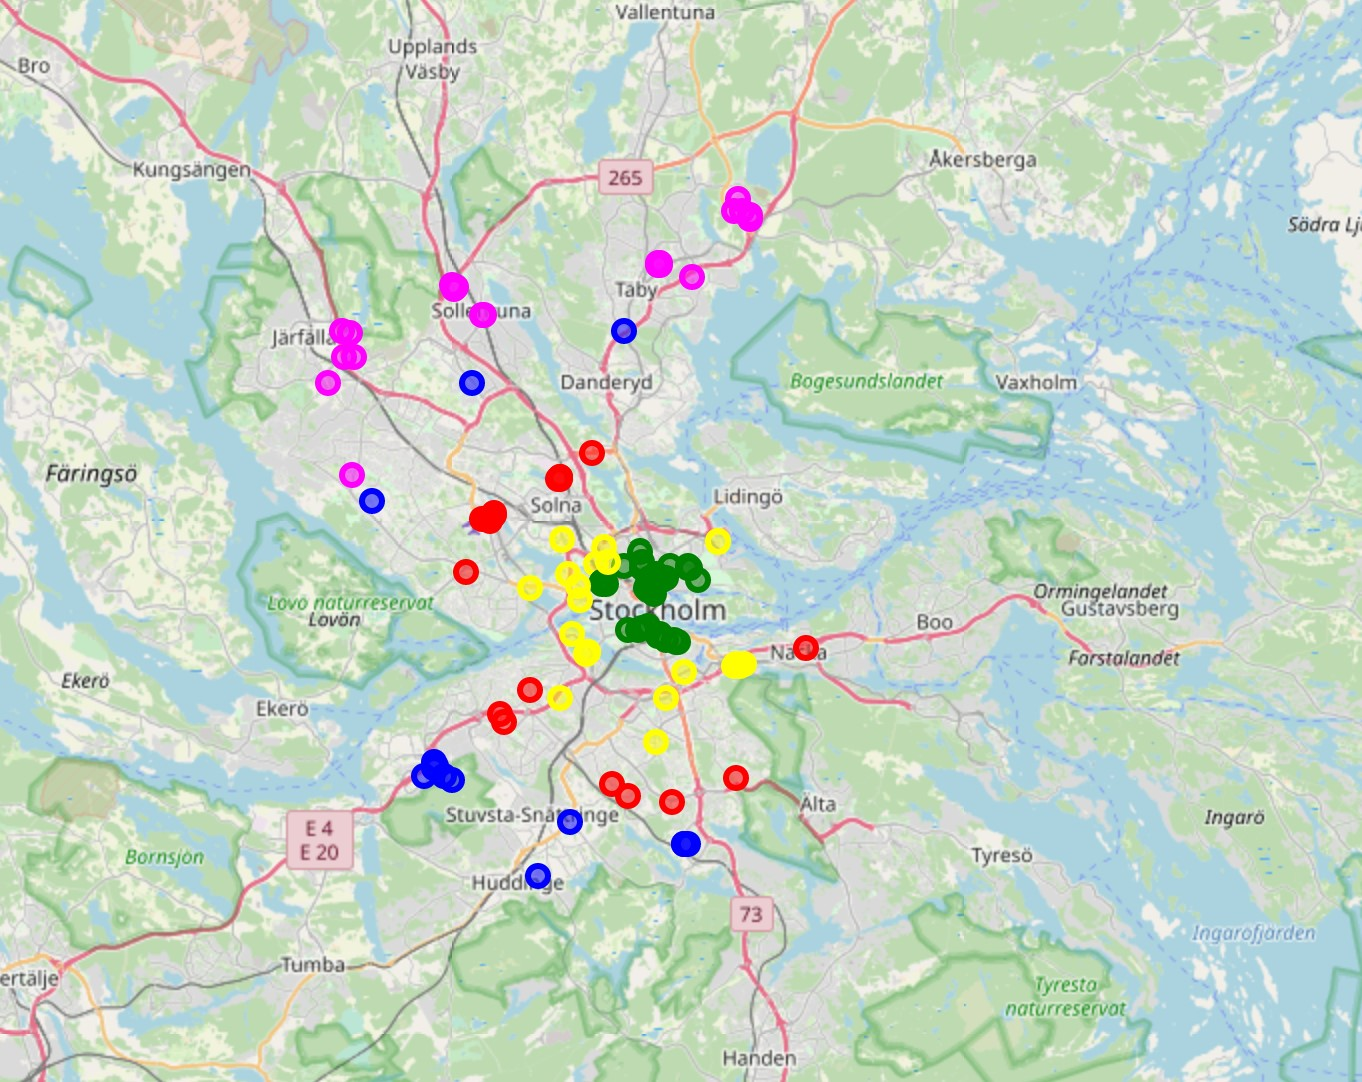
\includegraphics[width=\textwidth]{img/map2.jpg}
			\caption{Venues map after applying K-Means. In this case, each colour represent a cluster}
			\label{fig::map2}
		\end{figure}
		
		After obtaining this clusters a further sub-clustering process was needed, such that each cluster would contain at least one venue of each category. Two options were briefly explored. These will be explained briefly with the pros and cons of each one:
		
		\subsubsection{DBSCAN clustering}
		
		DBSCAN is a clustering algorithm that finds clusters within a data set based on "dense" regions. These dense regions are specified by the parameters of the DBSCAN function provided by sci-kit learn. These parameters include the minimum numbers of data points to be considered a cluster as well as the radius around each data point within which, other data points residing inside will be considered of the same cluster. All other data points that does not reside within a cluster, will be considered as "noise" this is, not useful information.
		The pros of using DBSCAN are:
		\begin{itemize}
			\item The function provided by sci-kit learn is easy to implement and tune.
			\item Given the way that DBSCAN determines clusters, it filters out less-dense areas.
			\item It is very easy to select the minimum amount of venues that have to be within a cluster.
			\item Computing time with this kind of small data sets is very low.
		\end{itemize}
		The cons of DBSCAN in this case are:
		\begin{itemize}
			\item It cannot be ensured that the clusters will have all the venue categories required straight out of the DBSCAN function.
			\item If a solution if found with this algorithm, it is not guaranteed that it is a global optimum solution.
			\item Some extra processing is needed to see if the clusters found are useful.
		\end{itemize}
		
		In order to simplify the coding complexity, DBSCAN was tested and deemed good enough for this study, therefore chosen as the second clustering algorithm. However, the second option might be more accurate and more suitable for either a larger study or a tool presented to end-users where it will be repeatedly used.
		\subsubsection{Manual development of algorithm}
		\label{subsec::MA}
		The second option was to develop a clustering algorithm, where for each of the KMeans clusters, all of the possible combinations $\binom{n}{5}$ where $n$ is the number of venues in a given KMeans cluster is stored in a list. Then, combinations that does not have the 5 different venue categories are removed from said list. Afterwards, the mean distance within venues in each combination is calculated and only a certain number, for example, the 5 combinations (New clusters) with the lowest mean distance are selected.
		
		The pros of this algorithm are:
		\begin{itemize}
			\item It guarantees to find global optimum solution
			\item Since only some of the combinations are selected, noise is also filtered out.
			\item Clusters formed are guaranteed to have the one and only one venue per category
		\end{itemize} 
		The cons of this algorith are:
		\begin{itemize}
			\item The coding complexity is greatly increased
			\item Some set operations might be difficult to achieve since they have to be done between different dataframes, lists, sets, etc.
			\item Computing time can increase, since the number of combinations increases very rapidly as the KMeans cluster number increases.
		\end{itemize}	
		
		Since the complexity of coding this algorithm is larger than the DBSCAN option, it was decided not to develop it.
		
	\subsection{Post-Processing of clusters}
	
	After obtaining the clusters with the DBSCAN algorithm, they were analysed to see how many of them complied with the requirements. It was found that only two of which did. One of them had already one venue per category, and the other had more than one venue in some of the categories. Therefore some cleanup was needed. Said cleanup can be seen in the jupyter notebook provided. In the following image, these clusters can be seen circled in red and the label given by the DBSCAN algorithm is put next to them. The grey points are the venues without cluster therefore considered as noise.
	
	\begin{figure}[H]
		\centering
		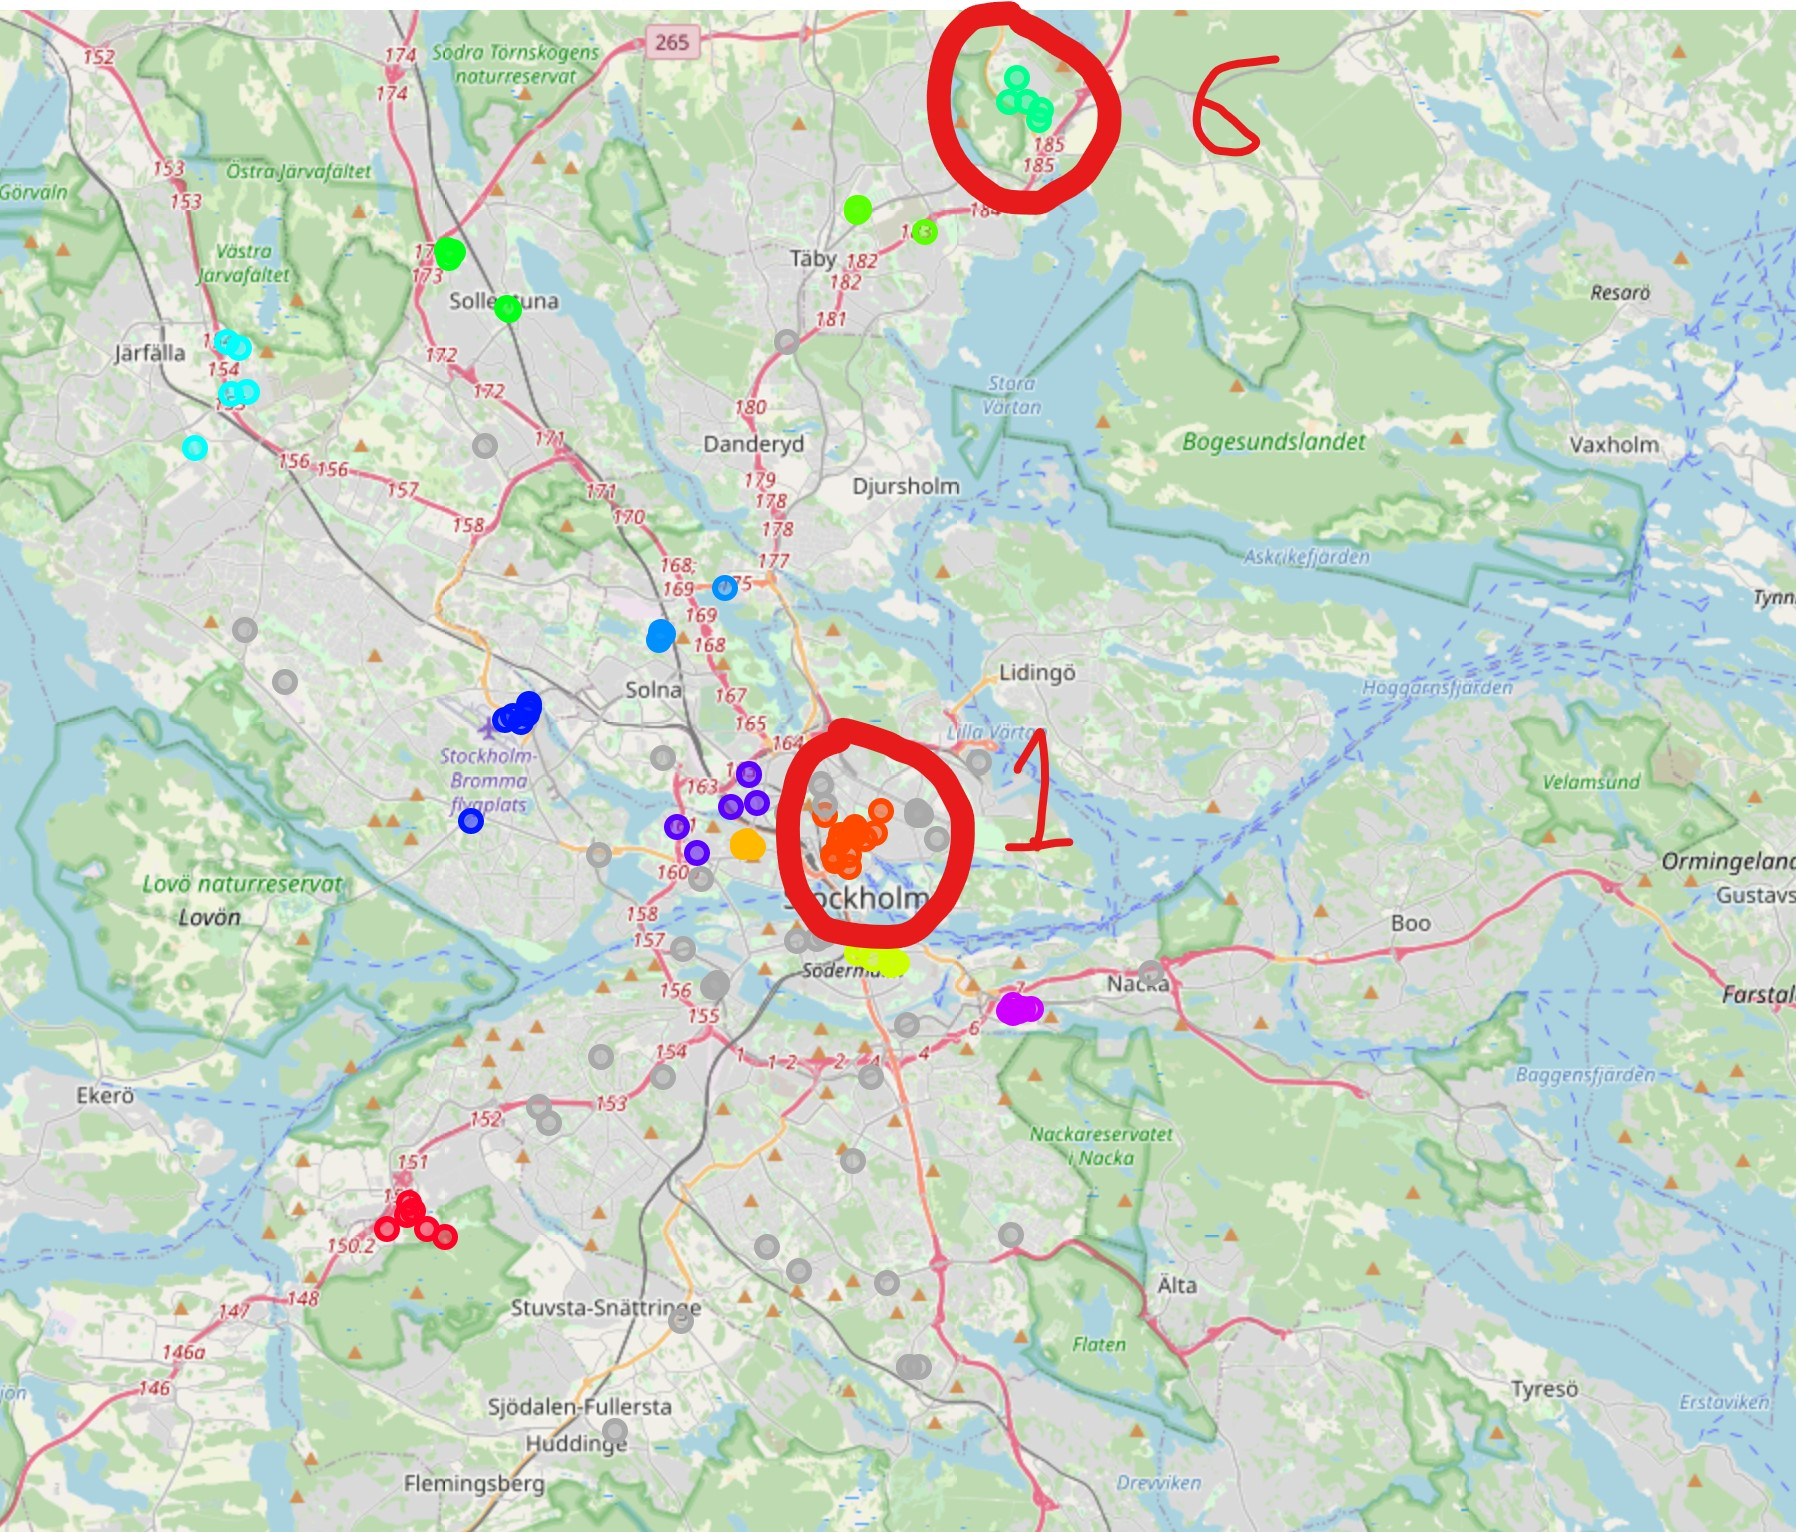
\includegraphics[width=\textwidth]{img/map3.jpg}
		\caption{Clusters obtained with DBSCAN}
		\label{fig::map3}
	\end{figure}
	
	As seen in the previous map (\ref{fig::map3}) it can be seen the two complying clusters. First, for cluster with label 1, it was reduced so that only one venue per category was included. This was done by taking the venue rating if available, or arbitrarily if not. 
	\subsection{Final Cluster selection}
	
	After the clusters had the same amount of venues (5). a simple weighted score was used:
	\begin{align*}
		\left(0.8 \cdot R_{avg}+0.2 \cdot 10\cdot \left(1-\frac{D_{avg}}{D_{Max}}\right)\right)=\left(0.8 \cdot R_{avg}+2 \cdot \left(1-\frac{D_{avg}}{D_{Max}}\right)\right)
	\end{align*}
	where $R_{avg}$ is the average rating of the venues in the cluster, $D_{max}$ is the maximum distance that the user was willing to travel for the shopping, in kilometres and $D_{avg}$ is the average distance of the clusters to the starting point.
	\newpage
\section{Results}
	The use of the scoring formula shown in the previous chapter resulted as follows: \\
	Cluster number 1 obtained a score of \textbf{7.18} out of 10.
	\newline
	Cluster number 6 obtained a score of \textbf{6.88} out of 10.
	\newline
	\newline
	
	This means that the best cluster to shop the initial items is cluster 1. For more details, please refer to the provided jupyter notebook.
	This result shows, that using machine learning can be used to recommend shopping areas for a wide variety of items and situations.
\section{Discussion}
	Throughout the development of these study, several recommendations were noted:
	\begin{itemize}
		\item If no fitting clusters were found with the DBSCAN algorithm, the one discussed in \ref{subsec::MA} must be used
		\item If enough computing power is available, a calculation with the second algorithm described of the combinations $\binom{n}{5}$ with n being all of the venues can be made. However, it might be computationally less efficient.
	\end{itemize}
\section{Conclusion}
	Studies like this can show the importance of the development of machine learning tools. While some specific cases can be seen as very simple, a tool like the one presented and developed here can be very powerful and useful, for example, when looking at shop clusters and the city where the user is looking for these shops is not well-known for any number of reasons, like just moved in, or if the user is in vacation.
	\newline
	\newline
	
	This work also provided excellent insight into the CRISP-DM process and how iterative it is, as very often it was required to go back in the notebook to do some other data cleaning or data acquirement because it was deemed necessary. Same when applying the machine learning algorithms as they often need a few iterations to find the correct parameters for each specific study. Needless to say, it is very important to know how each parameter modifies the behaviour and output of the algorithm since this can reduce the number of iterations needed.
	
	
	
	
	
	
	
\end{document}
